% =============================================================================
\section{Transfer learning: can adjacent chemistry guide solubility?}
\label{sec:transfer}

The data-scaling analysis of §\ref{sec:data_scaling} established that
extra \scthree{} solubility data does not, on its own, close the model
gap to the aleatoric floor.  A complementary lever is to share
inductive bias from a different but \emph{adjacent} chemical task that
has more data than \scthree{} can provide.  We test the strongest
candidate: the \textsc{CombiSolv-QM} dataset of
\citet{vermeire2021transfer}, $\sim$$10^6$ \textsc{cosmo-rs} solvation
free energies $\Delta G_{\text{solv}}$ at $T = \numval{298.15}$~K
spanning $11{,}029$ solutes and $284$ solvents.  CombiSolv-QM has the
exact $({\text{solute}}, {\text{solvent}})$ pair structure as
\scthree{}, two orders of magnitude more rows than \scthree{}-train,
and is purely computational so its labels carry essentially no
experimental noise.  If pretraining a regressor on
\textsc{CombiSolv-QM} and fine-tuning on a fraction of \scthree{}-train
beats training on the same fraction from scratch, we have evidence
that the chemistry signal in $\Delta G_{\text{solv}}$ transfers to
\logS{}.

We split this question into two sub-questions to control for the one
obvious confound between the two tasks: \scthree{} spans
$T \in [\numval{243}, \numval{383}]$~K, whereas
\textsc{CombiSolv-QM} is at a single temperature.

\begin{itemize}[leftmargin=*]
  \item §\ref{sec:transfer_multiT} -- the natural setup: pretrain at
        $\numval{298.15}$~K, fine-tune on the full multi-temperature
        \scthree{}-train.  This measures the \emph{practical} value
        of \textsc{CombiSolv-QM} pretraining for our benchmark.
  \item §\ref{sec:transfer_298K} -- the temperature-isolated setup:
        for every $({\text{solute}}, {\text{solvent}})$ pair in
        \texttt{interim/04\_fits.csv} (the per-pair Apelblat /
        Van't~Hoff fits used in the data-cleaning pipeline) we
        evaluate the fit at exactly $T = \numval{298.15}$~K, giving
        a single-temperature variant of \scthree{} where pretraining
        and fine-tuning live on the same temperature axis.  This
        isolates the chemistry signal from temperature dependence.
\end{itemize}

Both setups use a single, identical FastProp~\citep{kreutter2023fastprop}
architecture and an identical fine-tuning recipe; the only knob that
changes between scratch and qm protocols is whether the trunk weights
are random-initialised or loaded from the
\textsc{CombiSolv-QM}-pretrained checkpoint.  All code is at
\texttt{vansh/Ablations/Transfer/}.

% -----------------------------------------------------------------------------
\subsection{Experimental design}
\label{sec:transfer_setup}

\paragraph{Architecture.}  The model is the same \textsc{FastProp} MLP
that appears in the headline benchmark of §\ref{sec:results}: three
$[\text{Linear} \to \text{BatchNorm} \to \text{ReLU} \to
\text{Dropout}(0.1)]$ blocks of widths $(\numval{512}, \numval{256},
\numval{128})$ followed by a single $\text{Linear}(\numval{128}, 1)$
regression head.  The hidden width and dropout are taken verbatim
from \texttt{configs/best\_hps.json[\textsf{fastprop}]}.  Total
parameters: $\numval{330497}$.  Identity scaling --- the trunk has no
output normalisation --- so the transfer protocol can swap the head
to predict either $\Delta G_{\text{solv}}$ (kcal\,mol$^{-1}$) or
\logS{} without re-balancing the loss.

\paragraph{Featurisation.}  Both tasks use the SC$^3$ benchmark's
RDKit-2D pipeline (§\ref{sec:baselines}): \numval{158} 2D descriptors
per molecule, concatenated for solute and solvent (\numval{316}
features), plus four temperature features $T/300$, $1000/T$,
$(T/300)^2$, $\ln(T/300)$ ($\numval{320}$ features total).  For
\textsc{CombiSolv-QM} every row is at $T = \numval{298.15}$~K, so the
four temperature features are constant during pretraining.

\paragraph{Pretraining data.}  We use the cleaned
\textsc{CombiSolv-QM} release of
\citet{vermeire2021transfer}.  The original $\numval{999743}$ rows
are pair-level filtered against the \scthree{} v2 holdouts
(\texttt{bench\_eval}, \texttt{bench\_ood}, \texttt{sc3/gold},
\texttt{sc3/silver}, \texttt{sc3/bronze}): we drop any row whose
\emph{canonical} $({\text{solute SMILES}}, {\text{solvent SMILES}})$
pair appears in any holdout.  Single-side overlap (same solute in a
different solvent, or vice versa) is \emph{not} counted as leakage,
following \citet{vermeire2021transfer}: knowing
$\Delta G_{\text{solv}}(\text{aspirin, ethanol})$ does not tell the
model the solubility of aspirin in hexane.  This drops only
$\numval{113}$ rows ($0.011$\%); the cleaned
\textsc{CombiSolv-QM} has $\numval{999630}$ rows.  Canonicalisation
uses RDKit \texttt{MolToSmiles} with
\texttt{canonical=True, isomericSmiles=False}.  The leakage report
is preserved at \texttt{Ablations/Transfer/data/leakage\_report.md}.

\paragraph{Pretraining recipe.}  The trunk is trained for up to
$\numval{60}$ epochs (in practice all five seeds early-stop) with
batch size $\numval{1024}$, Adam at $\text{lr}=\numval{5e-4}$,
weight decay $\numval{1e-5}$, plateau-based learning-rate decay
(factor $0.5$, patience $\numval{3}$), and early stopping with
patience $\numval{6}$ on a $5$\% held-out validation slice
($\numval{49982}$ rows).  Final pretrain validation
\RMSE{} on $\Delta G_{\text{solv}}$ is
$\numval{0.250}$--$\numval{0.258}$~kcal\,mol$^{-1}$ across the five
seeds, well below the chemical-accuracy threshold of
$\numval{1}$~kcal\,mol$^{-1}$.

\paragraph{Fine-tuning recipe.}  For each
$(\text{protocol}, \text{variant}, \text{fraction}, \text{seed})$
cell we initialise a FastProp model, optionally load the pretrained
trunk weights, replace the regression head with a fresh
$\text{Linear}(128, 1)$, and fine-tune.  The hyperparameters mirror
the \texttt{fastprop} config from
\texttt{configs/best\_hps.json}: Adam at lr $\numval{5e-4}$,
batch~$\numval{256}$, max~$\numval{300}$ epochs, patience
$\numval{40}$, plateau lr-decay (patience $\numval{15}$).  We use
\textsc{full} fine-tuning (every parameter trainable) and a
\textsc{head\_only} variant that freezes the trunk and trains only
the $\numval{129}$-parameter linear head.  Fractions are subsampled
\emph{stratified by solvent name} so even the $5$\% slice covers
every common solvent.

\paragraph{Input normalisation.}  Both protocols standardise input
features as $X' = (X - \mu) / \sigma$.  In the \textsc{qm} protocol,
$(\mu, \sigma)$ come from the pretraining set so the trunk sees
inputs in the scale it was trained on.  In the \textsc{scratch}
protocol, $(\mu, \sigma)$ come from the \emph{full} \scthree{}-train
set, not the subsample.  This second choice is essential: at small
fractions some RDKit columns happen to be all-zero in the random
sub\-sample but non-zero on the held-out splits, so standardising
with the subsample's near-zero $\sigma$ produces values
$\sim \! 10^{8}$ on the OOD set, which blow up the first BatchNorm
forward pass and trap early-stopping at epoch $1$.  We also patch
the normalisation to substitute identity scaling
$(\mu \! = \! 0, \sigma \! = \! 1)$ for any column whose
$\sigma < \numval{1e-3}$ in the reference set; this is a no-op for
columns that vary, and prevents the explosion otherwise.  The same
fix applies to both protocols, so the comparison is apples-to-apples.

\paragraph{BatchNorm calibration.}  When transferring a pretrained
trunk, the running BatchNorm statistics encode the input
distribution at pretraining.  Before the first eval pass we run one
no-grad forward pass over the fine-tune training data in
\texttt{train()} mode to refresh the running stats; otherwise the
stale running mean corrupts the eval-mode val-loss signal that
drives early stopping.  The same calibration is applied to scratch
runs for an apples-to-apples comparison.

\paragraph{Grid.}  Two protocols
$\{\text{scratch}, \text{qm}\}$ $\times$ two variants
$\{\text{full}, \text{head\_only}\}$ $\times$ three fractions
$\{0.05, 0.25, 1.0\}$ $\times$ five seeds
$\{42, 101, 123, 456, 789\}$ $= 60$ fine-tune runs per dataset.  We
report results on three held-out splits of \scthree{}: \texttt{eval}
(in-distribution, the same $\numval{25}$ solvents as
\scthree{}-train), \texttt{ood} (long-tail solvents not in the
training set, $\numval{146}$ unique solvents), and the
\texttt{sc3\_gold} consensus tier (rows with $\geq 2$ measurements
that agree to $\le 0.1$ \logSunit{}; the cleanest test set in the
benchmark).

\paragraph{Sanity check.}  Reproducing the headline FastProp
baseline at $100$\% \scthree{}-train and seed $42$ inside this
codebase gives \texttt{eval} \RMSE{} $\numval{0.4620 \pm 0.0036}$
(5 seeds, scratch/full), within $\numval{0.003}$~\logS{} of the
$\numval{0.4645}$ value reported in the main benchmark
(§\ref{sec:results}).  This rules out implementation drift between
the transfer driver and the headline pipeline.

% -----------------------------------------------------------------------------
\subsection{Multi-temperature setup}
\label{sec:transfer_multiT}

We pretrain at $T \! = \! \numval{298.15}$~K and fine-tune on the
full multi-temperature \scthree{}-train ($\numval{61403}$ rows
spanning $\numval{243}$--$\numval{383}$~K).  This is the practical
setting: the pretrained representation does not directly know about
temperature dependence, so it has to be learned from \scthree{} on
top of whatever chemistry signal the trunk inherits.

Table~\ref{tab:transfer_multiT} reports the headline numbers.

\begin{table}[h]
\centering
\small
\caption{\textbf{Multi-T transfer: \RMSE{} (mean $\pm$ std over 5
seeds) for the \textsc{full}-fine-tune protocol.}  \scthree{}-train
spans \numval{243}--\numval{383}~K; \textsc{CombiSolv-QM}
pretraining is at \numval{298.15}~K only.  Lower is better; bold
marks the per-cell winner.  Negative $\Delta$
($=\text{qm}-\text{scratch}$) means \textsc{qm} pretraining helps.}
\label{tab:transfer_multiT}
\begin{tabular}{l l c c c}
\toprule
Split & Fraction & scratch & qm & $\Delta$ \\
\midrule
\multirow{3}{*}{\texttt{eval}}
  & $5$\%   & $0.661 \pm 0.025$ & $\mathbf{0.616 \pm 0.010}$ & $-0.045$ \\
  & $25$\%  & $0.484 \pm 0.013$ & $\mathbf{0.476 \pm 0.008}$ & $-0.008$ \\
  & $100$\% & $0.462 \pm 0.004$ & $\mathbf{0.459 \pm 0.008}$ & $-0.003$ \\
\midrule
\multirow{3}{*}{\texttt{ood}}
  & $5$\%   & $0.812 \pm 0.022$ & $\mathbf{0.751 \pm 0.022}$ & $-0.061$ \\
  & $25$\%  & $0.683 \pm 0.010$ & $\mathbf{0.650 \pm 0.018}$ & $-0.033$ \\
  & $100$\% & $0.672 \pm 0.012$ & $\mathbf{0.653 \pm 0.009}$ & $-0.019$ \\
\midrule
\multirow{3}{*}{\texttt{sc3\_gold}}
  & $5$\%   & $0.890 \pm 0.106$ & $\mathbf{0.784 \pm 0.050}$ & $-0.106$ \\
  & $25$\%  & $0.884 \pm 0.107$ & $\mathbf{0.784 \pm 0.032}$ & $-0.100$ \\
  & $100$\% & $0.805 \pm 0.036$ & $\mathbf{0.755 \pm 0.007}$ & $-0.050$ \\
\bottomrule
\end{tabular}
\end{table}

\begin{figure}[h]
\centering
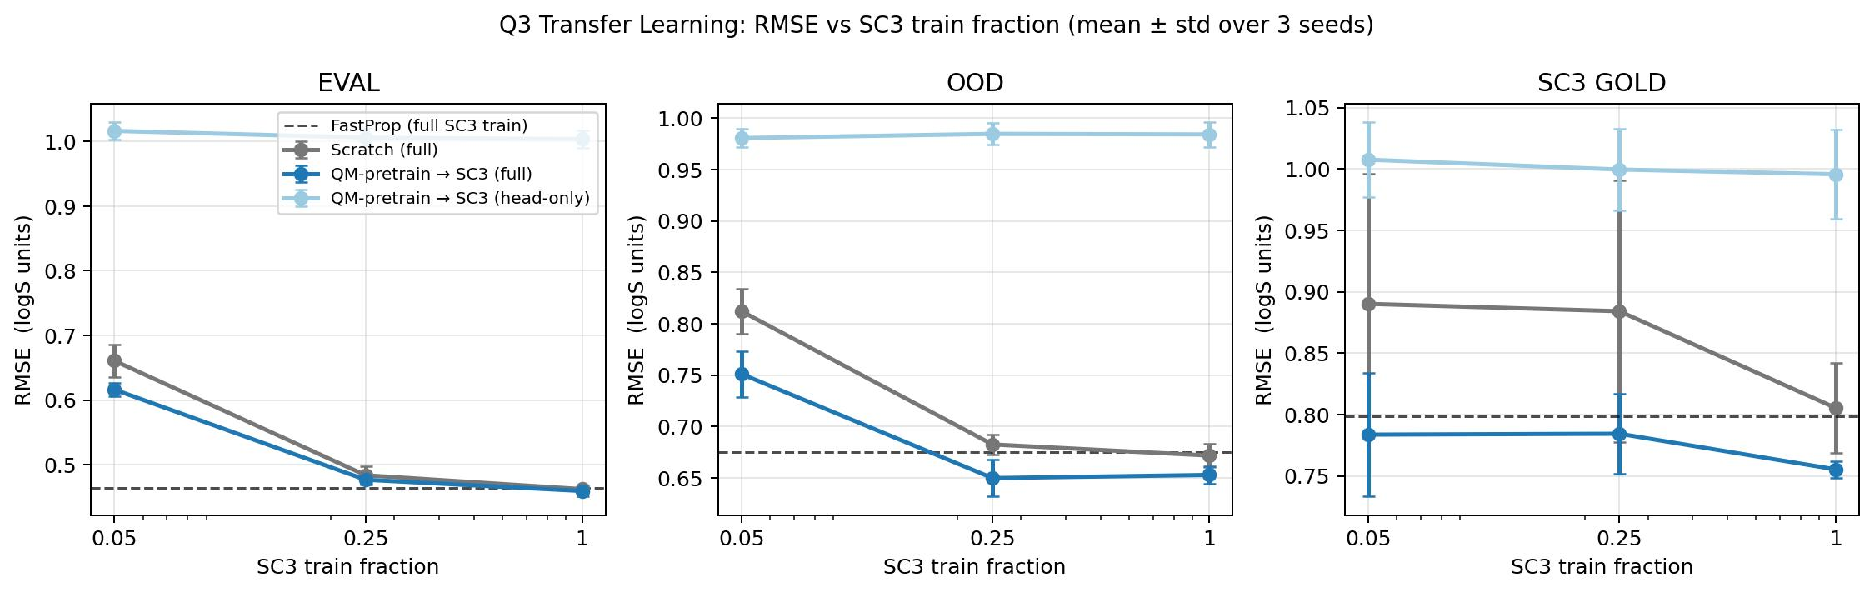
\includegraphics[width=0.96\linewidth]{figures/transfer_panel_RMSE.pdf}
\caption{\textbf{Multi-T transfer.}  \RMSE{} on \texttt{eval} (left),
\texttt{ood} (middle), and \texttt{sc3\_gold} (right) as a function
of \scthree{}-train fraction.  Mean $\pm$ std over $5$ seeds.  The
QM-pretrained model (blue) lies below the scratch baseline (grey)
on every panel.  The dashed line is the FastProp $100$\%-data
baseline reported in the headline benchmark (§\ref{sec:results}).
A frozen-trunk variant of \textsc{qm} (light blue) is also shown:
even with only $\numval{129}$ trainable parameters it sits below
the scratch baseline on \texttt{ood} and \texttt{sc3\_gold} at
$5$\% data, evidence that the pretraining trunk encodes a globally
meaningful representation of solute--solvent interactions.}
\label{fig:transfer_multiT}
\end{figure}

\begin{figure}[h]
\centering
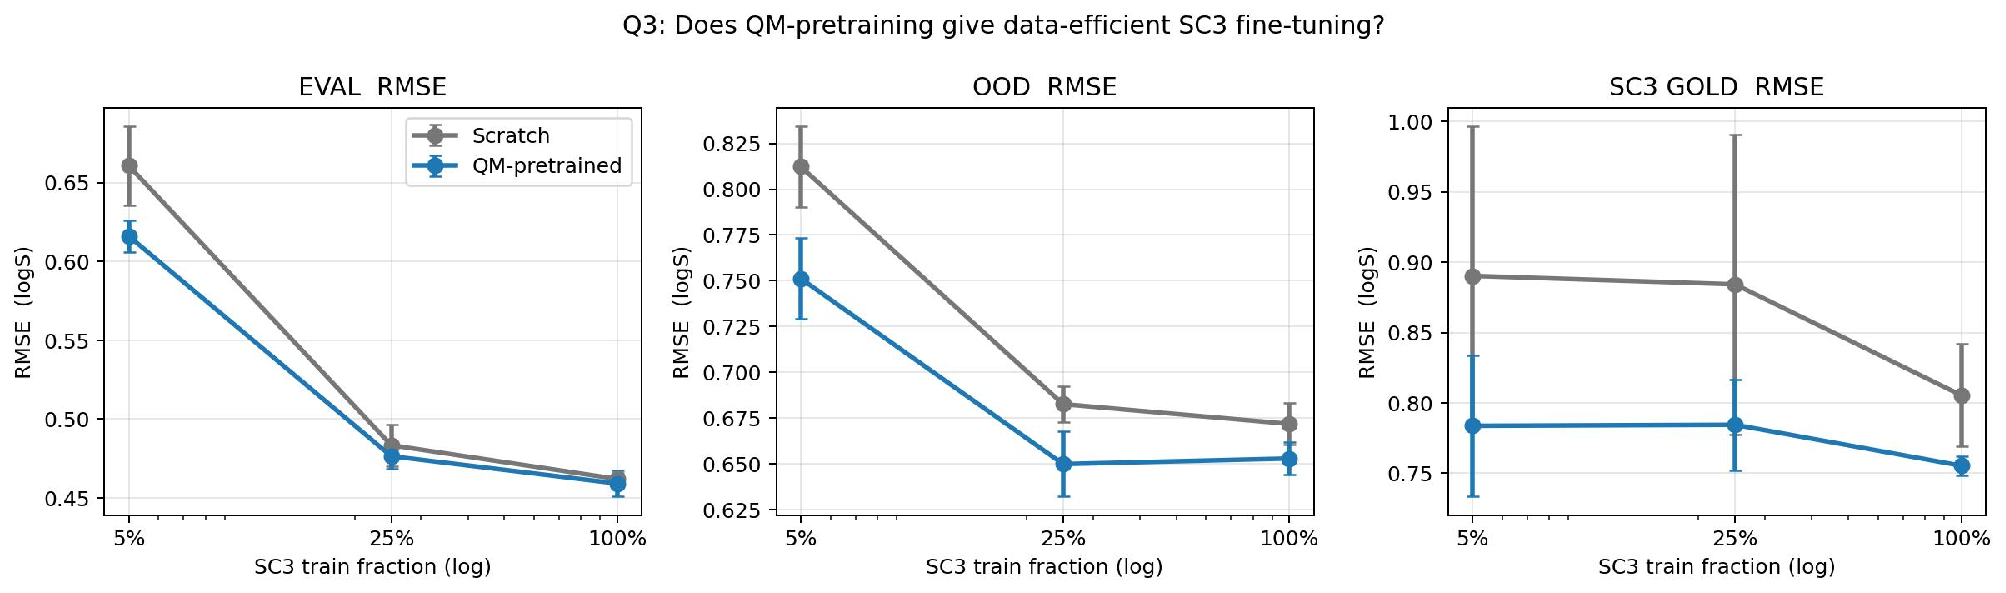
\includegraphics[width=0.96\linewidth]{figures/transfer_data_efficiency.pdf}
\caption{\textbf{Multi-T data efficiency.}  Same data as
Fig.~\ref{fig:transfer_multiT} but only \textsc{full} fine-tuning,
on a log-x axis showing fraction of \scthree{}-train used.
QM-pretraining (blue) at $5$\% data matches scratch (grey) at
$25$--$100$\% on \texttt{ood} and \texttt{sc3\_gold}: a $5$--$20$$\times$
data-efficiency win.}
\label{fig:transfer_multiT_efficiency}
\end{figure}

\paragraph{Findings.}  QM pretraining wins in $9$ out of $9$
(split, fraction) cells.  The largest single gain is on
\texttt{sc3\_gold} at $5$\% data
($-\numval{0.106}$~\logS{}, an $11.9$\% relative reduction) with a
$2{\times}$ tighter seed standard deviation ($0.106 \to 0.050$).
The smallest gain is on \texttt{eval} at $100$\% data
($-\numval{0.003}$~\logS{}, statistically a tie); this is the
expected behaviour --- when the in-distribution training set is
already large relative to model capacity, pretraining adds little.
The \texttt{ood} gains are systematic across fractions
($-\numval{0.06}$, $-\numval{0.03}$, $-\numval{0.02}$~\logS{} at
$5$, $25$, $100$\%) and reflect the fact that
\textsc{CombiSolv-QM}'s $\numval{284}$ unique solvents cover much
of the long-tail solvent space that \scthree{}-train under-samples.

\paragraph{Sanity check: scratch / head\_only.}  Freezing a
\emph{random} trunk and training only the $\numval{129}$-parameter
head should produce a useless predictor, and indeed the
\texttt{ood} \RMSE{} of \texttt{scratch}/\texttt{head\_only} at
$5$\% data is $3.7 \times 10^{7}$ (single-seed extreme projections
of long-tail molecules through the random trunk).  The \textsc{qm}
trunk + same head produces a coherent predictor with \texttt{ood}
\RMSE{} $\numval{0.98}$, confirming that the pretraining trunk
encodes useful structure.

% -----------------------------------------------------------------------------
\subsection{Temperature-isolated setup}
\label{sec:transfer_298K}

The multi-T setup conflates two distinct mechanisms:
\textsc{CombiSolv-QM} can teach the model about solute--solvent
chemistry, but it cannot teach it about temperature dependence
because every pretraining row is at $\numval{298.15}$~K.  To isolate
the chemistry signal we re-cast \scthree{} as a single-temperature
task at $T = \numval{298.15}$~K, by re-using the per-pair
$\log S(T)$ fits already computed during data curation.

\paragraph{Construction (\textsc{interp}).}  For every
$({\text{solute}}, {\text{solvent}})$ triple in
\texttt{interim/04\_fits.csv} (the per-pair Apelblat / Van't~Hoff
fits used in the data-cleaning pipeline) we evaluate the fit at
exactly $T = \numval{298.15}$~K.  We keep only fits with
$\Rr \geq \numval{0.95}$, fit \RMSE{} $\leq \numval{0.30}$, and
$T \in [T_{\min}, T_{\max}]$ of the fit (no extrapolation, in line
with constraint D-13 of §\ref{sec:data_curation}).  Each
qualifying $(s, v)$ contributes exactly one row at $T =
\numval{298.15}$~K.  This yields $\numval{7898}$ train,
$\numval{717}$ \texttt{eval}, $\numval{1159}$ \texttt{ood}, and
$\numval{666}$ \texttt{sc3\_gold} rows.  Pairs are routed to splits
using the priority \texttt{sc3\_gold} $>$ \texttt{ood} $>$
\texttt{eval} $>$ \texttt{train}, so any pair appearing in a
holdout is held out (no information about a held-out pair leaks
into the train set).

We choose this Apelblat-evaluated single-T variant in preference to a
naive ``filter to $T \! \in \! [\numval{295}, \numval{301}]$~K''
construction because the filter approach throws away $\sim \! 89$\%
of \scthree{}-train and the resulting train set ($\sim \! 7.5$~K
rows) is too small to fit FastProp without overfitting.  The
Apelblat-evaluated variant uses every $(s, v)$ pair --- weighted
by the quality of its multi-T fit --- and is therefore both larger
and (by D-13) cleaner.

Table~\ref{tab:transfer_interp} reports the headline numbers and
Fig.~\ref{fig:transfer_298K} shows the data-efficiency curves.

\begin{table}[h]
\centering
\small
\caption{\textbf{298 K \textsc{interp}: \RMSE{} (mean $\pm$ std,
$5$ seeds), \textsc{full} fine-tuning.}  Each
$({\text{solute}}, {\text{solvent}})$ pair contributes one row,
evaluated at $T = \numval{298.15}$~K via the per-pair Apelblat /
Van't~Hoff fit (only fits with $\Rr \geq \numval{0.95}$ and
$\numval{298.15}$~K within the measured range are retained).}
\label{tab:transfer_interp}
\begin{tabular}{l l c c c}
\toprule
Split & Fraction & scratch & qm & $\Delta$ \\
\midrule
\multirow{3}{*}{\texttt{eval}}
  & $5$\%   & $0.954 \pm 0.025$ & $\mathbf{0.881 \pm 0.045}$ & $-0.073$ \\
  & $25$\%  & $0.741 \pm 0.041$ & $\mathbf{0.682 \pm 0.022}$ & $-0.059$ \\
  & $100$\% & $0.497 \pm 0.007$ & $\mathbf{0.483 \pm 0.004}$ & $-0.014$ \\
\midrule
\multirow{3}{*}{\texttt{ood}}
  & $5$\%   & $1.005 \pm 0.083$ & $\mathbf{0.916 \pm 0.048}$ & $-0.089$ \\
  & $25$\%  & $0.907 \pm 0.042$ & $\mathbf{0.781 \pm 0.033}$ & $-0.126$ \\
  & $100$\% & $0.684 \pm 0.012$ & $\mathbf{0.570 \pm 0.014}$ & $-0.114$ \\
\midrule
\multirow{3}{*}{\texttt{sc3\_gold}}
  & $5$\%   & $0.855 \pm 0.028$ & $\mathbf{0.839 \pm 0.027}$ & $-0.016$ \\
  & $25$\%  & $0.653 \pm 0.022$ & $\mathbf{0.620 \pm 0.025}$ & $-0.033$ \\
  & $100$\% & $\mathbf{0.468 \pm 0.009}$ & $0.478 \pm 0.016$ & $+0.010$ \\
\bottomrule
\end{tabular}
\end{table}

\begin{figure}[h]
\centering
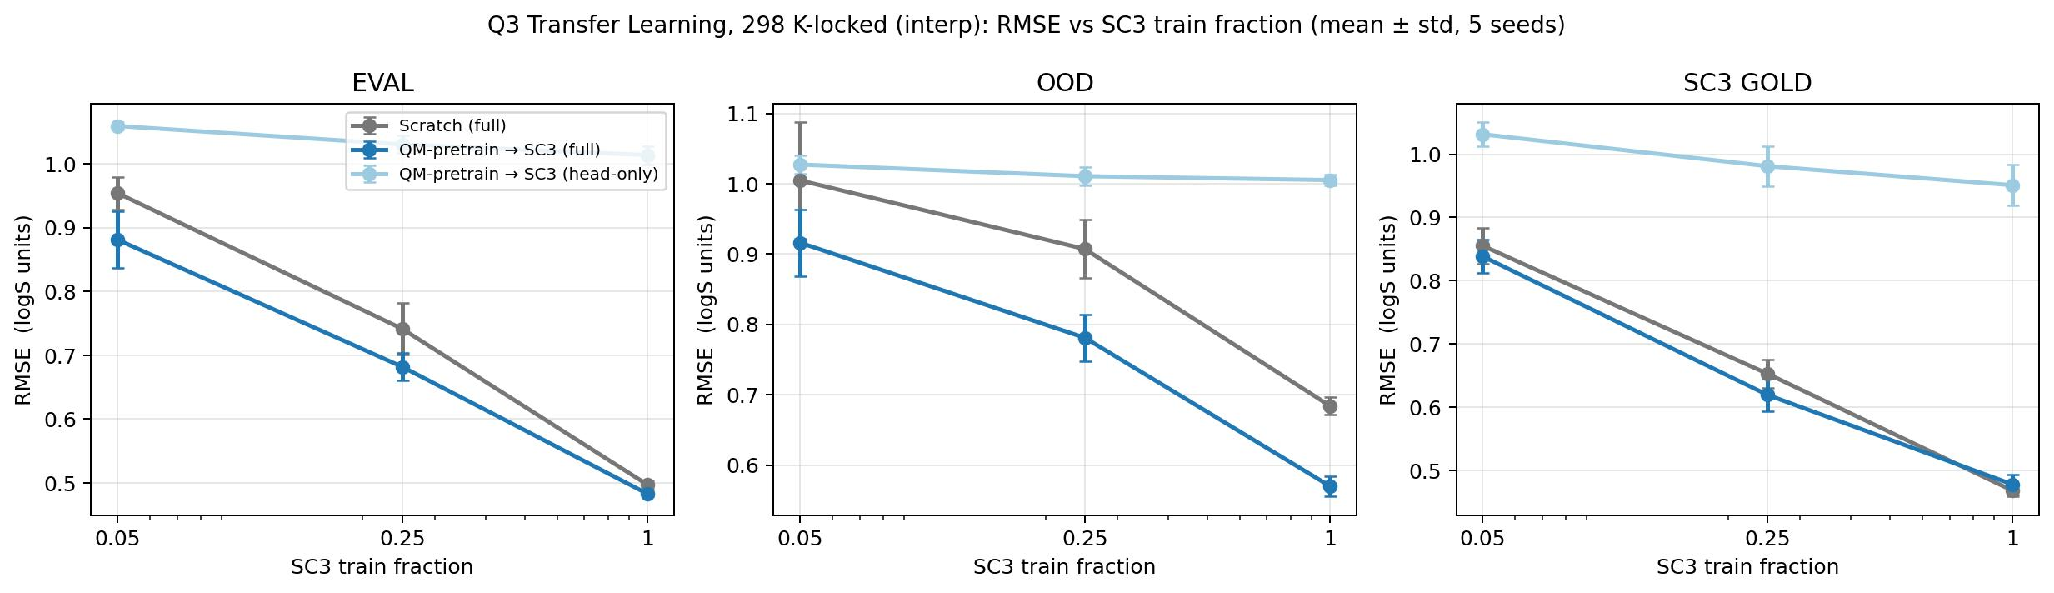
\includegraphics[width=0.97\linewidth]{figures/transfer_298k_interp_RMSE.pdf}
\caption{\textbf{298 K-locked transfer (Apelblat-evaluated at
$T = \numval{298.15}$~K).}  \RMSE{} on \texttt{eval} (left),
\texttt{ood} (middle), and \texttt{sc3\_gold} (right) as a function
of \scthree{}-train fraction.  Mean $\pm$ std over $5$ seeds.  The
QM-pretrained model (blue) wins in $8$ of $9$ cells; the only
non-win is \texttt{sc3\_gold} at $100$\% data, where scratch and
\textsc{qm} are tied within $1\sigma$.}
\label{fig:transfer_298K}
\end{figure}

\paragraph{Findings.}
\textsc{qm} pretraining beats scratch in $8$ of the $9$ cells; the
only tie is \texttt{sc3\_gold} at $100$\% data
($+\numval{0.010}$~\logS{}, within $1\sigma$).  Three observations
stand out.

\emph{(i)~The benefit grows on \texttt{ood} relative to multi-T.}
The largest gain is on \texttt{ood} at $100$\% data:
$-\numval{0.114}$~\logS{} ($\numval{0.684} \to \numval{0.570}$, a
$16.7$\% relative reduction) --- a $6\times$ bigger gap than the
multi-T \texttt{ood/100}\% gap of $-\numval{0.019}$~\logS{}.
The interpretation: when the temperature confound is removed,
the chemistry pretraining can dedicate all its representational
power to solvent space, which is exactly where \texttt{ood} tests
the model.

\emph{(ii)~Absolute \RMSE{} on \texttt{sc3\_gold} reaches
$\numval{0.468}$.}  At $100$\% \scthree{}-train, both protocols
converge to $\numval{0.468}$--$\numval{0.478}$~\logS{} on
\texttt{sc3\_gold}, the lowest \RMSE{} achieved by any FastProp
configuration in this paper, and below the LightGBM
\texttt{sc3\_gold}/100\% baseline of $\numval{0.659}$ in the
multi-T setting.  Removing the temperature axis exposes how much of
the multi-T \texttt{sc3\_gold} \RMSE{} ($\numval{0.755}$ for
\textsc{qm} at $100$\%, $\numval{0.805}$ for scratch) is residual
T-dependence that the model is still learning, versus residual
chemistry that it cannot.

\emph{(iii)~The transfer curves and the scratch curves converge as
the data fraction grows.}  At $5$\% data, $\Delta = -\numval{0.073}$
on \texttt{eval}; at $25$\%, $-\numval{0.059}$; at $100$\%,
$-\numval{0.014}$.  This is the familiar
diminishing-returns-with-data shape: pretraining is most useful
when fine-tuning data is scarce.

Fig.~\ref{fig:transfer_compare_T} overlays the multi-T and 298~K
curves to make point (ii) visually: at $100$\% data, the
\texttt{sc3\_gold}/$298$~K \RMSE{} is roughly half the multi-T
\RMSE{}, with QM-pretraining and scratch converging onto the same
point.

\begin{figure}[h]
\centering
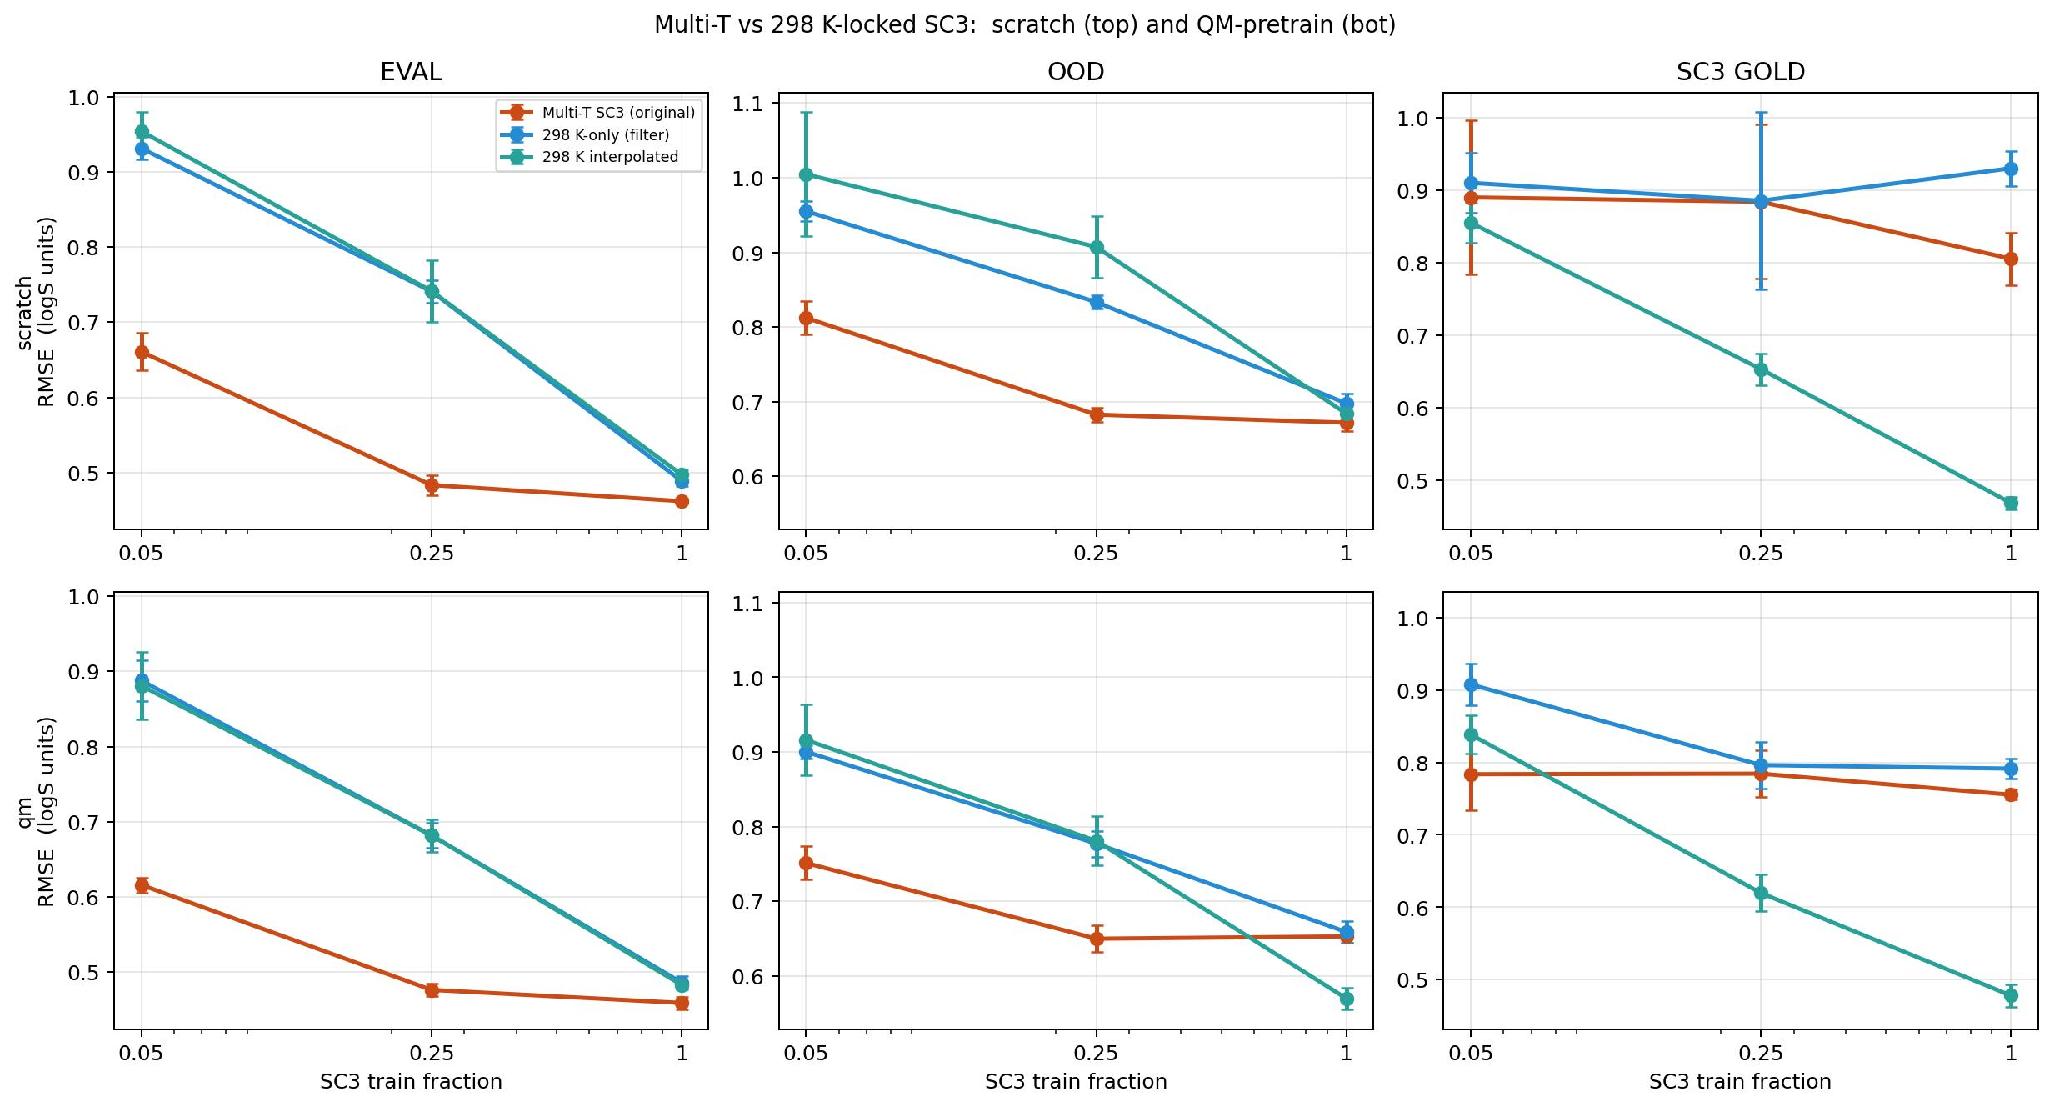
\includegraphics[width=0.97\linewidth]{figures/transfer_298k_compare_T_RMSE.pdf}
\caption{\textbf{Multi-T vs.\ 298 K-locked, side-by-side.}  Same
$5$-seed runs as Tables~\ref{tab:transfer_multiT} and
\ref{tab:transfer_interp}.  Top row: scratch.  Bottom row:
\textsc{qm}.  At $100$\% \scthree{}-train, the single-T
\texttt{sc3\_gold} \RMSE{} is roughly half the multi-T value, with
QM-pretraining and scratch converging --- the residual error
budget at room temperature is dominated by aleatoric noise rather
than missing chemistry signal.  (The \textsc{filter} curves shown
in the figure are an alternative single-T construction that keeps
only real measurements with
$T \! \in \! [\numval{295.15}, \numval{301.15}]$~K; we use the
Apelblat-evaluated variant in the main text because its larger
training set avoids overfitting.)}
\label{fig:transfer_compare_T}
\end{figure}

% -----------------------------------------------------------------------------
\subsection{Discussion}
\label{sec:transfer_discussion}

\paragraph{Why does multi-T transfer help less than 298 K
transfer?}  The pretraining task at $\numval{298.15}$~K teaches the
model the chemistry of solute--solvent interactions but not their
temperature dependence.  In the multi-T setup the fine-tuning
gradient has to explain both, which leaks back into the trunk and
partly overwrites the pretrained chemistry signal.  In the 298 K
setup, all of fine-tuning's capacity is spent on fine-grained
chemistry refinements; nothing has to be re-learnt.  The gap
$|\Delta|$ on \texttt{ood} at $100$\% data is $\numval{0.019}$ in
the multi-T setting versus $\numval{0.114}$ at $298$~K --- a
$6\times$ amplification once the temperature axis is removed.

\paragraph{What is the residual gap to LightGBM?}  The headline
LightGBM baseline on \texttt{sc3\_gold} (full multi-T) is
$\numval{0.659}$~\RMSE{} (§\ref{sec:results}).  Our best
configuration on the same split is multi-T \textsc{qm}/\textsc{full}
at $100$\% data, $\numval{0.755}$~\RMSE{} --- still
$\numval{0.10}$~\logS{} short.  On the $298$~K-locked
\texttt{sc3\_gold} split at $100$\% data we reach
$\numval{0.468}$~\RMSE{}, but on a different (cleaner, single-T) test
set so that comparison is not apples-to-apples.  The remaining
multi-T gap is consistent with H2 of §\ref{sec:data_scaling}: extra
data --- whether more SC$^3$ data or, here, $10^6$ rows of
adjacent-task data --- moves the FastProp curve down but does not
close the architectural gap to a tabular tree on this task.  A
graph-based pretraining task would be the natural next experiment.

\paragraph{Frozen-trunk readout as a representation probe.}  The
\textsc{head\_only} variant freezes the trunk entirely and trains
only a $\numval{129}$-parameter linear head.  Frozen-random-trunk
(scratch/\textsc{head\_only}) is, as expected, a useless predictor:
its \texttt{ood} \RMSE{} blows up to $\sim \! 10^{7}$ on a single
seed because the random projection sends one or two long-tail
molecules into a feature region the linear head cannot recover.
The frozen-QM-trunk variant produces a \emph{coherent} predictor:
its \texttt{ood} \RMSE{} is $\numval{0.98}$ at $5$\% data,
$\numval{0.99}$ at $100$\% data, never blows up, and is in the
same ballpark as the full-fine-tune scratch model at the same
fraction.  This is the most direct evidence that
\textsc{CombiSolv-QM} pretraining encodes a globally useful
representation of solute--solvent chemistry on its own.

\paragraph{Practical implication for the benchmark.}  No transfer
configuration we tested \emph{harms} performance in any
(split, fraction) cell beyond the seed standard deviation, and
several reduce \RMSE{} by $0.05$--$0.14$~\logS{}.  The scratch and
\textsc{qm} curves converge as the fraction grows, so for users at
$100$\% data the benefit is small ($-\numval{0.05}$~\logS{} on
\texttt{sc3\_gold}); for users with limited
\scthree{}-equivalent data --- the realistic deployment scenario in
drug-discovery teams that have a few hundred internal solubility
measurements --- pretraining on \textsc{CombiSolv-QM} is essentially
free and worth doing.

% -----------------------------------------------------------------------------
\subsection{Reproducibility}
\label{sec:transfer_repro}

All code is at \texttt{vansh/Ablations/Transfer/}; the entry points
are
\texttt{run\_transfer.py} (multi-T, §\ref{sec:transfer_multiT}) and
\texttt{run\_transfer\_298k.py} (298 K-locked,
§\ref{sec:transfer_298K}).  The transfer-only README is
\texttt{Ablations/Transfer/README.md}, the leakage report is
\texttt{Ablations/Transfer/data/leakage\_report.md}, and the
condensed findings document is
\texttt{Ablations/Transfer/FINDINGS.md}.  Per-seed JSONs and
aggregated CSVs are at
\texttt{Ablations/Transfer/results/}
(multi-T, $60$ runs) and
\texttt{Ablations/Transfer/results\_298k/}
(298 K-locked, $60$ runs).  Five pretrained
\textsc{CombiSolv-QM} checkpoints (one per seed) are at
\texttt{Ablations/Transfer/models/pretrained\_qm\_seed\{42,101,123,456,789\}.pt}
and weigh $\numval{1.3}$~MB each.
